\documentclass[a4paper]{book} % If you don't know LaTeX, ignore everything until \begin{document}
\usepackage[utf8]{inputenc}
\usepackage{graphicx}
\usepackage{avant}
\renewcommand{\familydefault}{\sfdefault}
\addtolength{\evensidemargin}{-2cm}
\addtolength{\textwidth}{2cm}
\begin{document}
\fontsize{24}{28}\selectfont
\title{Introduction to Communism}
\author{Matvei "LeftHandedLeftist" Ivanov \\ and Kris Karlov}
\date{Written in 2018}
\maketitle
\fontsize{24}{28}\selectfont
\chapter{What is communism?}
Communism is a system where the means of production are owned by the community. The means of production are the tools that are needed to produce something. For example, machines in a factory are means of production.

It is different from the system most of the world has now. That system is called capitalism. It lets certain people or groups own the means of production while all other people work for them.

\begin{figure}[tbhp]
\centering
\include[width=0.9\textwidth]{1-1.png}
\caption{Under communism, the workers decide how much of what to produce}
\end{figure}

Because the owners the means of production under capitalism, who are also called the bourgeoisie, want to continue owning them, they often spread lies about what communism is and what happens while we get to it.

Often, they say that communism is when everyone owns everything. This is wrong. Only the means of production are owned by the community. The things that aren't used to produce something, also called personal property, can still be owned by a single person. Someone can still own a watch or a bicycle under communism. But the factories that produce watches or bicycles are owned by the community.

Sometimes they also call anything the state does communism. This is also wrong. Actually, there is no state under communism. It just isn't necessary. There are no reasons to fight about the means of production because they're already owned by everyone. And if someone wants to get them for themselves or starts a fight about personal property, the community will resist them.

Very often they say that communism is impossible, that humans will naturally try to get the most for themselves and only themselves. But they're wrong. Early humans did not have a single group owning the means of production. It was better for them to help their community, because they couldn't live without it: the community defended each other against the many dangers that were there.

\begin{figure}[tbhp]
\centering
\include[width=0.9\textwidth]{1-2.png}
\caption{A group of early humans fighting a lion. Each of them couldn't do that alone, but in a strong community, they can.}
\end{figure}

Some say that the times have changed, the systems became more complicated, and communism can't exist now. It's true that it's not possible to immediately make a society communist now. This is why there is a step towards it called socialism. Socialism is possible, and it exists right now in a few countries.

\chapter{Why do we need communism?}

You see, the workers do almost all the work and the bourgeoisie do barely any. Even though the bourgeoisie does a small amount of work they get much much higher wages than the workers. We need to abolish (remove) this flaw. The best route is through SOCIALISM and COMMUNISM.

\begin{figure}[tbhp]
\centering

\includegraphics[width=0.9\textwidth]{2-1.png}
\caption{A bourgeois telling a worker where and how to work, while getting most of the money}
\end{figure}
  
  As we stated before, in communism the workers own the factories. Another great benefit of communism is the removal of money. This might sound silly; But you see, without money, there are no taxes and big projects (for example a new road) don't need money which means it can be done well and fast.

\begin{figure}[tbhp]
\centering
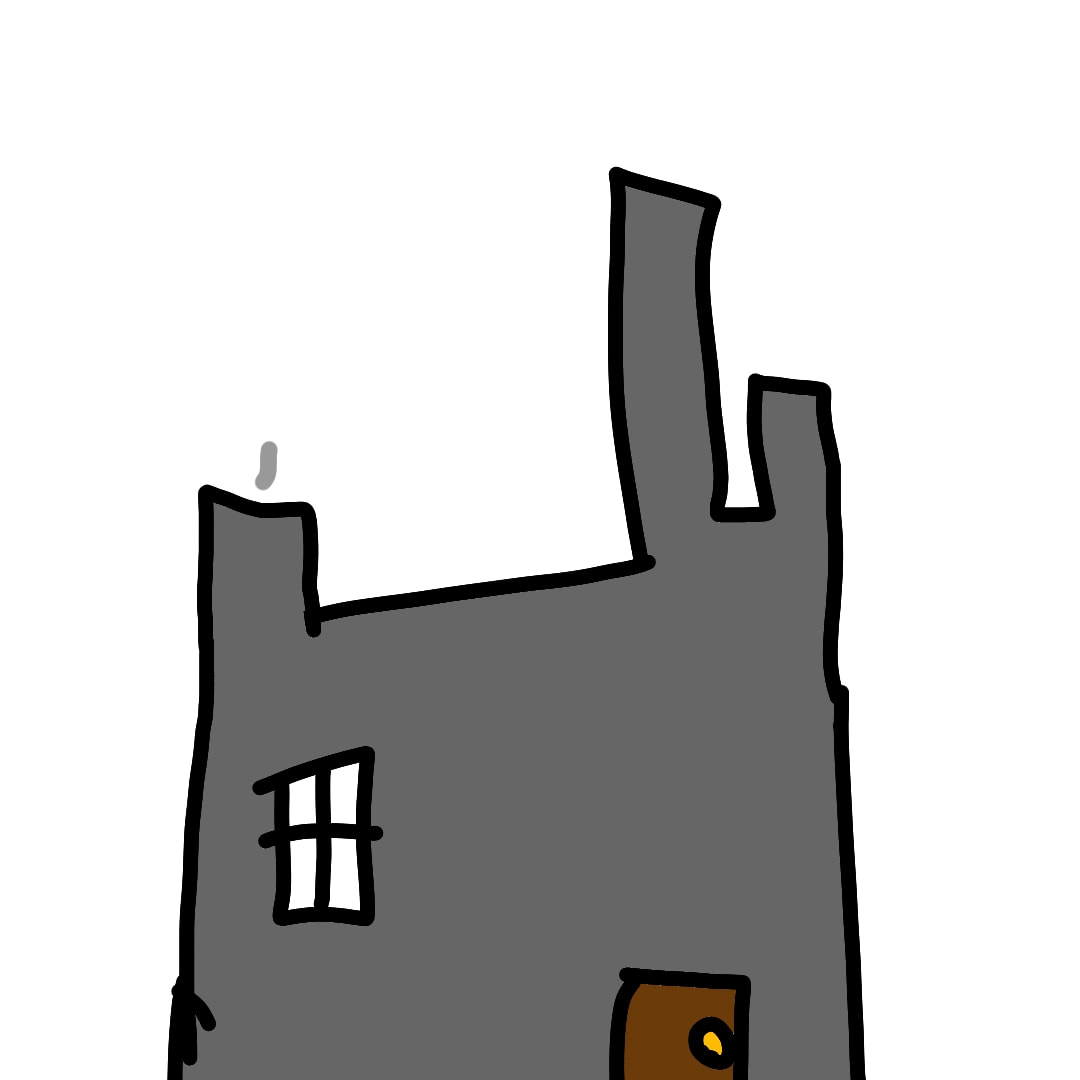
\includegraphics[width=0.9\textwidth]{2-3.png}
\caption{A factory, which is owned by the workers under communism and by the bourgeoisie under capitalism}
\end{figure}

  Under Communism, there is also no government. This is good because then the people must choose decisions.

\begin{figure}[tbhp]
\centering

\includegraphics[width=0.9\textwidth]{2-5.png}
\caption{Under communism, the people themselves decide. So the decisions actually make the people happy, not some small group richer.}
\end{figure}

  Before COMMUNISM there should be Socialism. Socialism has a planned economy which means that random spikes in costs do not happen. Socialism does have money in its early stages; But after it has labour vouchers. 

\begin{figure}[tbhp]
\centering
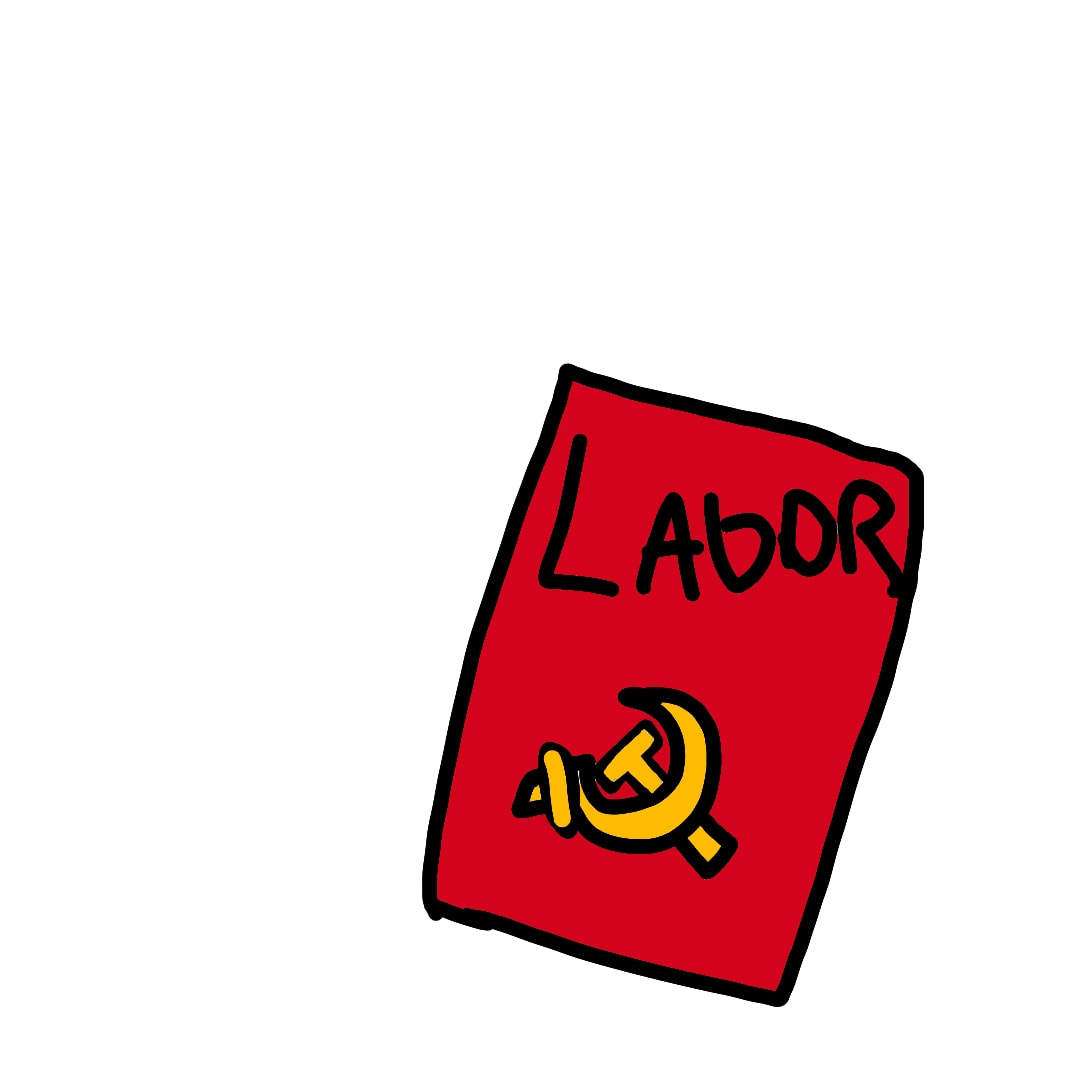
\includegraphics[width=0.9\textwidth]{2-4.png}
\caption{A labour voucher}
\end{figure}

  Labour vouchers are money that disappears after it is spent. This is so that people cannot make things extremely expensive and get huge profits. We might discuss this more in a later paper.

\end{document}
